\documentclass{standalone}
\usepackage{mintikz}

\begin{document}
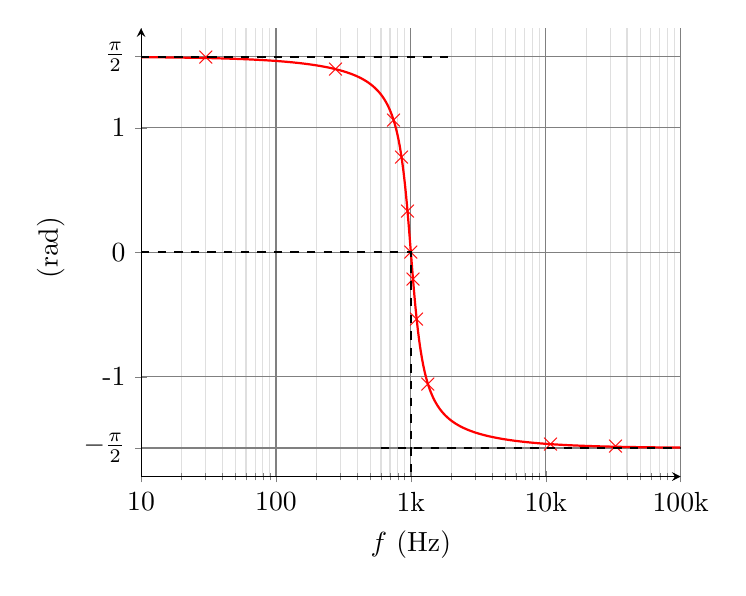
\begin{tikzpicture}[]
    \begin{semilogxaxis}[
        xmin=1e-2, xmax=1e2,
        ymin=-1.8, ymax=1.8,
        xlabel={$f$ (Hz)}, ylabel=$\f$ (rad),
        xtick={1e-2, 1e-1, 1e0, 1e1, 1e2},
        xticklabels={10, 100, 1k, 10k, 100k},
        ytick={-1.57079, -1, 0, 1, 1.57079},
        yticklabels={$\DS-\frac{\pi}{2}$, -1, 0, 1, $\DS\frac{\pi}{2}$},
        % extra y ticks={0.78539, 1.57079},
        % extra y tick labels={$\DS\frac{\pi}{4}$, $\DS\frac{\pi}{2}$},
        % extra y tick style={grid=none},
        axis lines=left,
        grid=both,
        major grid style={black!50},
        minor grid style={gray!25},
        clip=true]
        \def\Q{3}
        \addplot[
        domain=1e-2:1e2, samples=500,
        smooth, thick, red]
        {-atan(\Q*(\x-1/\x))*pi/180}
        node[pos=0.1] {$\times$}
        node[pos=0.3] {$\times$}
        node[pos=0.4] {$\times$}
        node[pos=0.43] {$\times$}
        node[pos=0.47] {$\times$}
        node[pos=0.5] {$\times$}
        node[pos=0.52] {$\times$}
        node[pos=0.55] {$\times$}
        node[pos=0.6] {$\times$}
        node[pos=0.8] {$\times$}
        node[pos=0.9] {$\times$}
        ;
        \addplot[
        domain=1e-2:2,
        smooth, black, dashed, thick]
        {pi/2};
        \addplot[
        domain=6e-1:1e2,
        smooth, black, dashed, thick]
        {-pi/2};
        \draw[dashed, thick]
        (axis cs:1e-2,0) -|
        (axis cs:1e0,-1.8);
    \end{semilogxaxis}
\end{tikzpicture}
\end{document}
